\section{Software artefacts}
\subsection{Ecore metamodel \& Xtext grammar}
The software artifacts we have implemented have been uploaded to the Modelia Git repository \cite{Tracea_Repo} and can be accessed in following URL:
\verb|https://github.com/modelia/tracea|

Folder \verb|\model| contains the Ecore metamodel, its corresponding Xtext grammar, and a set of well-formedness rules written in OCL. We also added the source for the running example we used to illustrate this report. Here are some adaptations we applied to fit the DSL on Eclipse-EMF~\cite{EMF}:
\begin{itemize}
    \item We added a class \texttt{Tracea} that acts as the root of the metamodel. A \texttt{Tracea} has a name and contains the set of \texttt{Artefacts}, \texttt{Traces}, \texttt{Evidences} and \texttt{RelationshipTypes} instantiated for cross-reference reuse. \textit{This class is the root containment for Ecore implementation. }
    \item We slightly relaxed \textit{containment references} to ease the manipulation of references with Xtext. Next iteration on the metamodel should take note of relaxing containment.
\end{itemize}
  
\begin{figure}[h]
	\centering 
	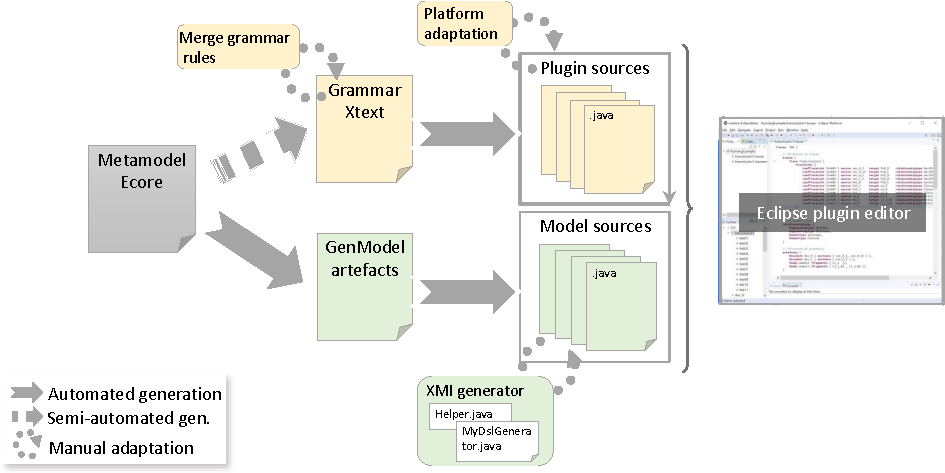
\includegraphics[width=.99\linewidth]{images/xtext-workflow}
	\caption{Xtext plugin development workflow}
	\label{fig:xtext-workflow}
\end{figure}

\subsection{Eclipse Xtext editor plugin for Tracea}
This deliverable contains a concrete syntax written in Xtext~\cite{xtext}. The source of this artifact has been uploaded with the DSL on Modelia Git repository. 
A set of six projects is part of the execution. In particular, \verb|\Tracea| contains the input artefacts: a metamodel in Ecore, and an Xtext file with its concrete grammar. The other five contain sources generated via Xtext Artefact generator on the EMF platform~\cite{EMF}. 

Xtext provides support for the parsing of the grammar. We developed a dedicated Eclipse editor for Tracea files and implemented a generator to save Tracea file in XMI format. 
Figure \ref{fig:xtext-workflow} describes the development of the plugin. EMF uses Ecore metamodel to generate a GenModel file and a set of source artefacts (visible in \verb|\Tracea\model\src|). We modify these files to generate a copy of Tracea files translated into XMI. The modification can be found in \verb|\Tracea\model\xtend-java-edit-for-XMI|. 
From an Xtext grammar, EMF generates an Eclipse plugin editor. Packages and source artefacts are created in \verb|uoc.som.tracea|, \verb|uoc.som.tracea.ide|, \verb|uoc.som.tracea.test|, \verb|uoc.som.tracea.test.ui|, and \verb|uoc.som.tracea.ui|. Depending on the environment of production, the importation of packages in the Xtext file may vary. The two different versions (with nsURI, or with path) are present at the top of the Xtext. To execute the plugin, a new instance of eclipse must be launched from \verb|uoc.som.tracea|. 

Figure \ref{fig:plugin} shows a screenshot of the Tracea editor. On the left hand, there is a file explorer and an outline (common Eclipse plugin views). On the right hand, an editor that colorizes keywords and spellchecks words. The plugin assists the user with auto-completion and verifies the grammar with the emission of warnings and errors.


\begin{figure}[ht] 
	\centering 
	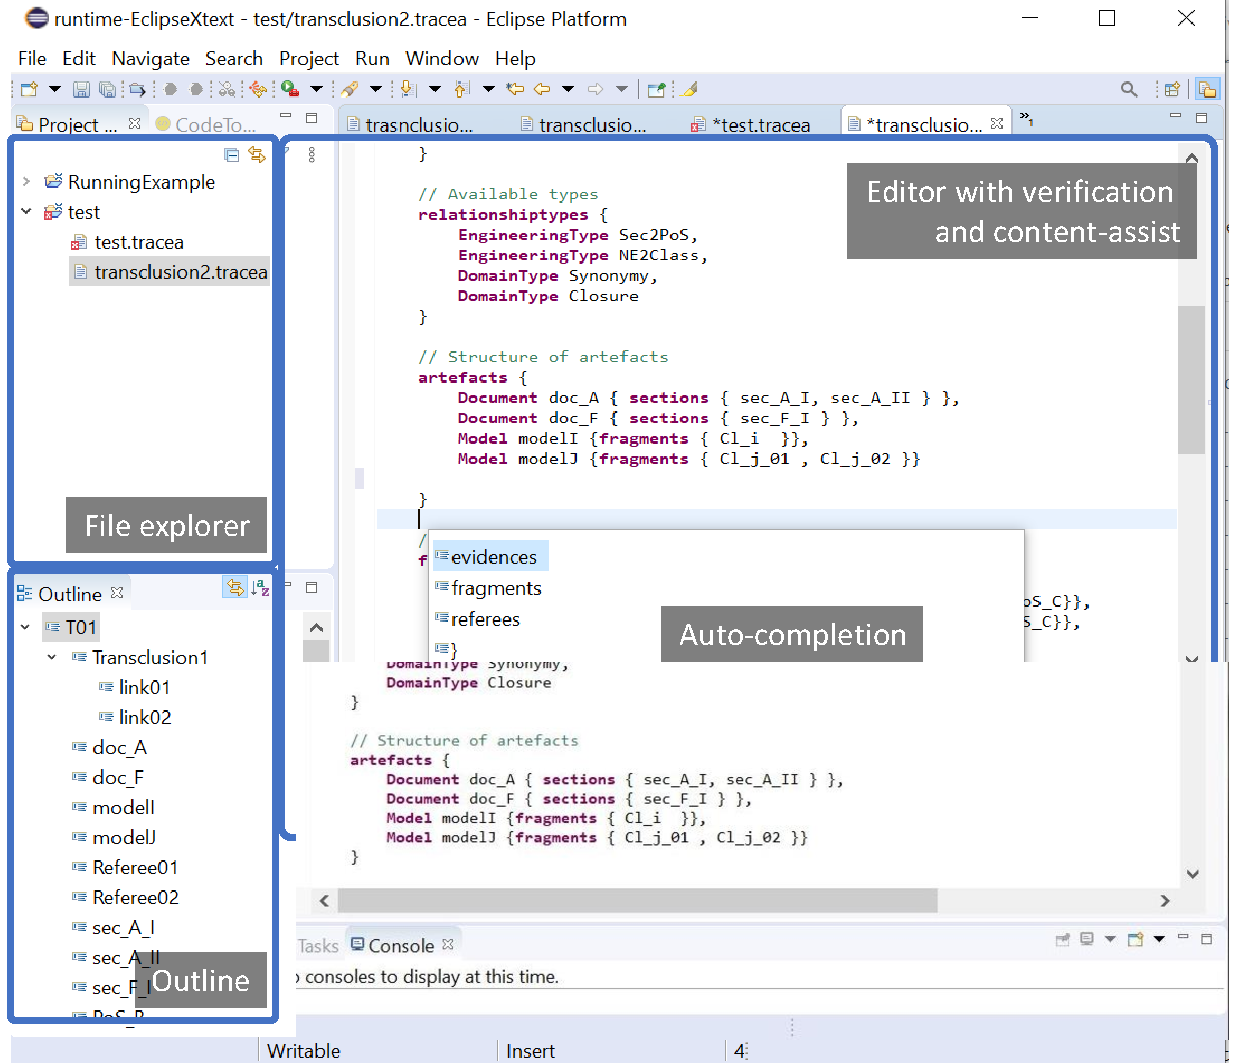
\includegraphics[width=.99\linewidth]{images/plugin-screenshot}
	\caption{Screenshot of the Tracea editor.}
	\label{fig:plugin}
\end{figure}
